\documentclass{article}

\usepackage{mathtools}
\usepackage{graphicx}

\begin{document}


\title{Examen parcial 1\\
	\large Computación}
\author{Tulio Muñoz Magaña}
\maketitle

La primera Parte del examen se encuentra en la carpeta de Primera parte.\\

\textbf{Segunda Parte}\\

\textbf{1.-} La función recibe dos apuntadores a caracteres, donde comienzan dos arrays. Lo que hace la función es copiar la segunda cadena ingresada a la primera.\\
Dentro del while tenemos una asignación. Una asignación se considera como expresión verdadera si el valor por la izquierda es distitnto de $0$, y falsa si no. Entonces, mientras el valor por la izquierda de lo que está dentro del while no sea $0$, la asignación se seguira ejecutando, junto con los incrementos de los apuntadores, que van recorriendo el array, y asignandol al primer array el caracter correspondiente del segundo. Cuando se acabe el segundo array habrá un $0$, que se pasará al primero y lo terminará, después de eso el while ya no seguirá porque el valor por la izquierda será $0$, y yatendremos en segundo array copiado al primero.\\

\textbf{2.-} El código da un error al compilarse, por la expresión *x++ que se encuentra en el printf. El compilador imprime bien los primeros $4$ valores, pero después se queda parado, la función tiene la intención de ir imprimiendo en pantalla los valores del array $x$ hasta encontrar un número mayor a $90$, entonces deja de imprimir.\\

\textbf{3.-} El error del programa es que se asigna $2*num$ a $res$. Pero $res$ es un apuntador a un flotante y $num$ es un flotante, por lo que hay una incompatibilidad de tipo de dato. Para solucionarlo tendríamos que acceder al contenido del lugar al que apunta $res$, lo cual lo haríamos con $*res = 2*num;$\\

\textbf{4.-} Un apuntador es un tipo de dato en donde se guarda una dirección de memoria que corresponde a un lugar donde se almacena otro tipo de dato. Por ejemplo el apuntador char* a; guarda la dirección de memoria de un lugar donde se almacena un caracter.\\

\textbf{5.-} Una variable global es aquella a la que se puede acceder desde cualquier lugar del programa, se definen fuera de cualquier contexto, y si no son inicializadas, se inicializan automáticamente en $0$. Las variables locales son definidas dentro de un contexto, y solo pueden ser accedidas dentro de ese contexto.\\

\textbf{6.-} El ejemplo se encuentra en la carpeta del examen.\\

\textbf{7.-} \textbf{Arquitectura de Von Neumann}\\

La arquitectura de Von Neumann es muy importante porque implementa la innovadora idea de almacenar en la memoria de la computadora no solo los datos, sino también los programas, y para eso se adopta la siguiente configuración: \\

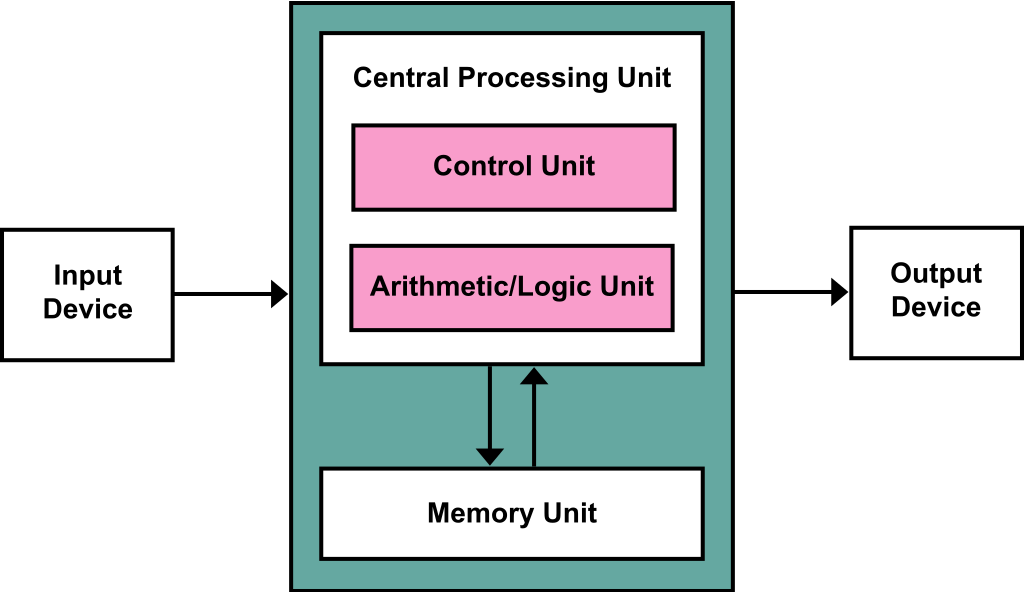
\includegraphics[width = \textwidth]{von}\\

El dispositivo de entrada recibe los datos del usuario, y el dispositivo de salida le comunica los resultados, ya sea medianta pantallas o algún otro mecanismo de salida.\\

La Unidad aritmético lógica de encarga de realizar los cálculos numéricos necesarios para llevar a cabo las tareas, como suma, resta, multiplicación, etc. Y operaciones lógicas como and y or. La unidad de control se encarga de decidir cuál será la tarea que se llevará a cabo a continuación, es la que orquesta la computadora. Estas dos unidades conforman la unidad central de procesamiento. Dentro de ésta se encuentran también los registros, que es una memoria de altísima velocidad, y muy baja capacidad, que se encarga de almacenar la información importante de uso inmediato, además de la dirección de memoria de la siguiente instrucción, de la instrucción que se está ejecutando, etc.\\

La memoria guarda los datos y las instrucciones, la unidad central de procesamiento se encarga de solicitarle la información que necesite al momento de realizar un algoritmo. \\

Las partes de la arquitectura se comunican mediante los buses, hay bus de datos, de control, de direcciones, y periféricos. El bus de datos lleva la información, el de control se encarga de llevar las indicaciones, y de direcciones pues lleva las direcciones y los buses periféricos se comunican con los dispositivos de entrada y salida. 













































\end{document}